\documentclass[]{article}
\usepackage[round]{natbib}

\usepackage{fullpage}
\usepackage{url}
\usepackage{authblk}
\usepackage{graphicx}
\usepackage{color}
\usepackage{booktabs}

% cross-reference with main text
\usepackage{xr}
\externaldocument{manuscript}

% local definitions
\newcommand{\aprcomment}[1]{{\textcolor{blue}{Comment: #1}}}

\title{Supporting Information}
\author{APR}
\date{\today}

\begin{document}
\maketitle

\section{Supplemental Figures}

\begin{figure}[ht!]
    \centering
    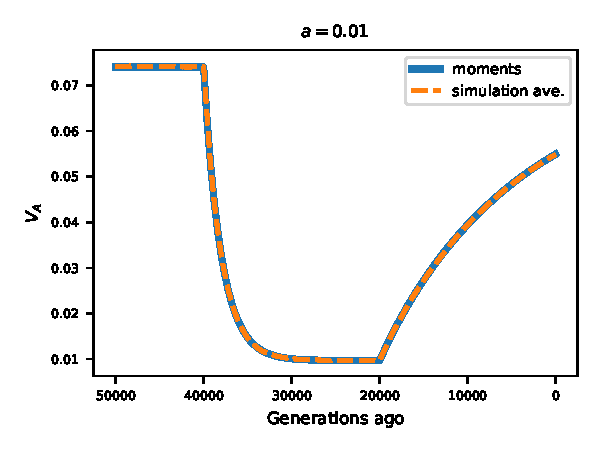
\includegraphics{../figures/one_pop.a_0.01.pdf}
    \caption{
        \textbf{Simulations assuming no linkage with weak effects.}
        All mutations have $a=0.01$.
    }
    \label{fig:one-popA}
\end{figure}

\begin{figure}[ht!]
    \centering
    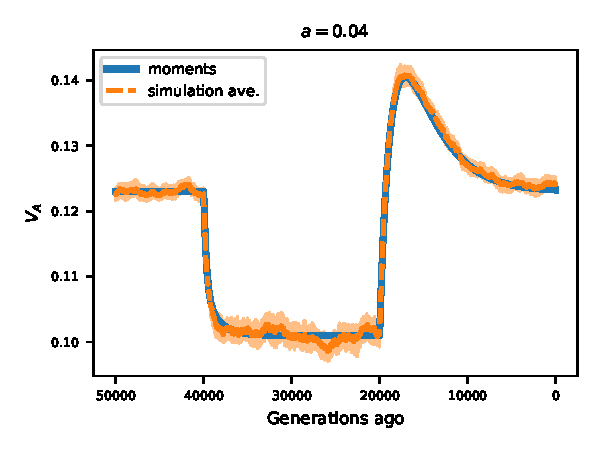
\includegraphics{../figures/one_pop.a_0.04.pdf}
    \caption{
        \textbf{Simulations assuming no linkage with moderate effects.}
        All mutations have $a=0.01$.
    }
    \label{fig:one-popB}
\end{figure}

\begin{figure}[ht!]
    \centering
    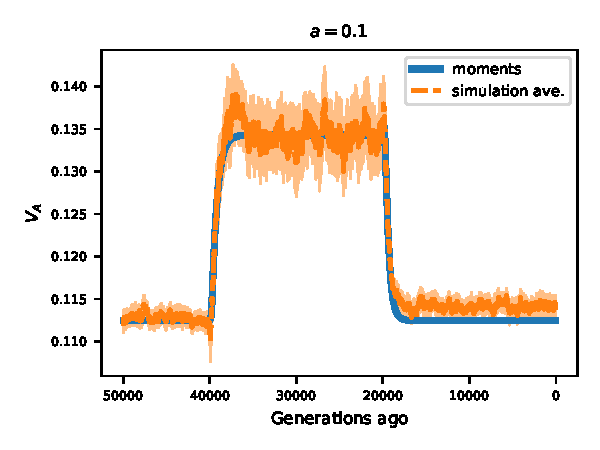
\includegraphics{../figures/one_pop.a_0.1.pdf}
    \caption{
        \textbf{Simulations assuming no linkage with strong effects.}
        All mutations have $a=0.1$.
    }
    \label{fig:one-popC}
\end{figure}

\begin{figure}[ht!]
    \centering
    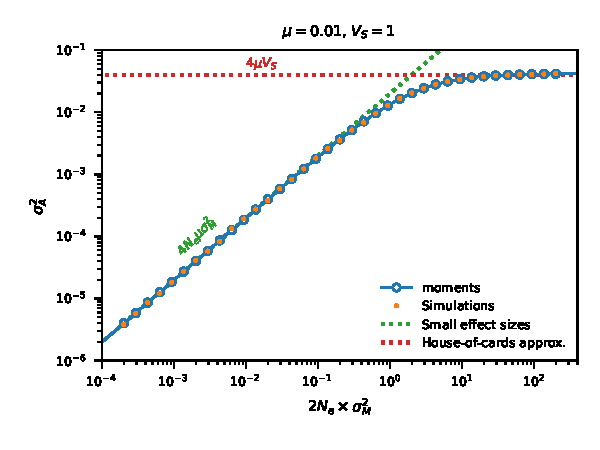
\includegraphics{../figures/vary_SD.pdf}
    \caption{
        \textbf{The Lande-Turelli continuum.}
    }
    \label{fig:turreli-lande}
\end{figure}
\end{document}
